\documentclass[11pt]{article}
\pdfinfoomitdate=1\pdftrailerid{}
\usepackage[letterpaper,margin=.7in,headheight=15pt,headsep=18pt,footskip=24pt]{geometry}
\usepackage[T1]{fontenc}
\usepackage{lmodern,amsmath,amssymb,array,booktabs,fancyhdr,tikz}
\renewcommand{\familydefault}{\sfdefault}
\setlength{\parindent}{0pt}\setlength{\parskip}{6pt}
\pagestyle{fancy}\fancyhf{}
\fancyhead[L]{\small Week 53 / Connecting networks / Adult return-visit guide}
\fancyfoot[L]{\scriptsize Bellingham Math Circle / Week 53 / W53-RV-FAC-v1}
\fancyfoot[R]{\thepage}
\renewcommand{\headrulewidth}{0pt}
\newcommand{\head}[1]{\par{\large\bfseries #1}\par}
\newcommand{\sub}[1]{\par\textbf{#1}\par}
\newcommand{\hint}[1]{\textit{Hint if needed.} #1}
\newcommand{\links}[1]{\ensuremath{\{\text{#1}\}}}
\begin{document}
\head{Mathematical overview}
\textbf{Model and first-visit facts.} Use a finite connected undirected map, whole printed links and strictly positive prices. Buying pays once per link; traveling pays for every traversal. Length on paper is not price. With every place required, a cheapest network is a tree, with $n-1$ links on $n$ places: a loop could lose a link and cost less. The first visit's other useful fact is the exchange certificate: a tree is cheapest exactly when no unused link is cheaper than a link on the tree route between its ends.

\textbf{Cheapest networks solve every lowest-dearest-route problem at once.} A route's \emph{dearest} link is its largest price, not its total. Every route along a cheapest all-place network has the smallest possible dearest price among routes with those endpoints. If a cheaper-dearest route existed, remove a dearest tree link. That separates the tree into two sides; the proposed route crosses the separation on a cheaper link, giving a cheaper tree. Conversely, a tree with this property for \emph{every} pair is cheapest, by the exchange certificate. Merely minimizing the largest price anywhere in the network is not enough.

\textbf{Opening links determines the price list and cost.} Open \emph{all} links priced at most $k$, not just a chosen network. The reachable groups only merge. Two places first share a group at exactly their lowest possible dearest price. Let $c_k$ be the number of groups and $c_0=n$. Every cheapest tree has exactly $n-c_k$ links priced at most $k$: its low-price pieces must join every group, by the preceding route fact, and each piece is a tree. Thus it has $c_{k-1}-c_k$ links of price $k$. All cheapest trees share one price list even when their links differ. For positive \emph{integer} prices,
\[
 \text{cheapest cost}=\sum_{k\ge1}k(c_{k-1}-c_k)=\sum_{k\ge0}(c_k-1).
\]
The sums stop when there is one group. Include thresholds at which nothing merges. This is an explanation of children's records, not a buying recipe to give them first.

\textbf{Trips and networks react differently to repricing.} Adding $a$ to every price adds $a(n-1)$ to every all-place tree, so it changes no cheapest network while prices stay positive. A trip of $j$ links gains $aj$, so different-length trips can overtake. Doubling preserves both kinds of optimum. More generally, strictly increasing repricing preserves all cheapest all-place trees, including ties, because it preserves every exchange comparison. Squaring positive prices can nevertheless change cheapest trips.

\textbf{Optional places change the problem.} Circles must connect; squares need not. A cheapest purchase has no loop and no optional leaf: either could be trimmed for a saving. With two required places it is a cheapest trip; with all places required it is the original tree problem. In between, a purchase can resist every cheaper single change yet not be cheapest. With $r\ge2$ required places, at most $r-2$ optional places can have three or more bought links; the leaf-count proof is on guide p.~8. The preceding all-place price-list, repricing and converse claims do \emph{not} extend to optional places.

\textbf{Discovery and evidence.} Building supplies examples; a failed search is not impossibility. A complete small catalog proves that case; the cut and leaf arguments explain general claims. K--1 compares reachable groups and optional-place payment piles (fixed maps: dots to 4, totals to 12). Grades 2--3 compares dearest links, sums and invented prices (printed comparisons to 18). Grades 4--5 connects catalogs to proofs and tests where local improvement fails. Reading and recording may be adult-supported; link choices stay with children.
\newpage
\head{Preparation and shared launch}
\textbf{Status.} Unpiloted and physically unrehearsed. Print scale, tape clearance, pawn fit, counter handling, preparation time and the proposed pacing still need a real rehearsal. Digital checks do not establish classroom readiness.

\textbf{Kit per pair or upper trio.} Reuse 30 equal counters about 12--15 mm across, ten removable tape strips about $5\times20$ mm, one small pawn or a finger, one sleeve and dry-erase pen, an off-map tray, and one sheet of scrap paper as a second payment area. The young and middle tables each have two kits (60 counters, 20 strips, two of each other item); the upper trio has one. Add 15 counters and four strips for demonstration: 165 counters and 54 strips overall. These are planning quantities for five working groups, not an attendance claim.

\textbf{Print and prepare.} US Letter, single-sided, 100\%. The return-visit files are \texttt{k-1.pdf} (7 pages), \texttt{grades-2-3.pdf} (6), and \texttt{grades-4-5.pdf} (10). Print selected pages once per pair/trio, not one full packet per child. The large maps are working mats; small duplicate maps and examples are pen-only records. Working place circles are 10 mm across, with centers roughly 40 mm or more apart. No pages are cut. Base Week 53 has \emph{no materials PDF}; no base student page is needed for the routes below. For an optional familiar comparison, print \texttt{week-53-students.pdf} p.~3 (trap) or p.~4 (five-place map) as an uncut mat. Current base guide: W53-guide-v4.

Allow a proposed 15--20 minutes to print selected mats, count kits and prepare strips; this estimate is unmeasured. Before class, place strips on the tightest map you will use. Keep price labels visible and counters off the roads. If a pawn hides a place, use a finger. Thirty counters cover the listed optimal single payments, \emph{not every possible purchase}: the squared-price map even has a price-36 link. Write large trial totals rather than demand an oversized payment pile. On the six-place comparisons, $18+15=33$ and $16+16=32$ exceed one kit: write the first total, return its counters, then pay the second.

\textbf{Whole group, about 5 minutes after free handling.} Draw this non-task line on the board; circles about 10 mm wide and centers at least 40 mm apart. Let a child choose and mark one whole link; show its payment, then finish the line. This is a convention example, not an optimization question.
\begin{center}
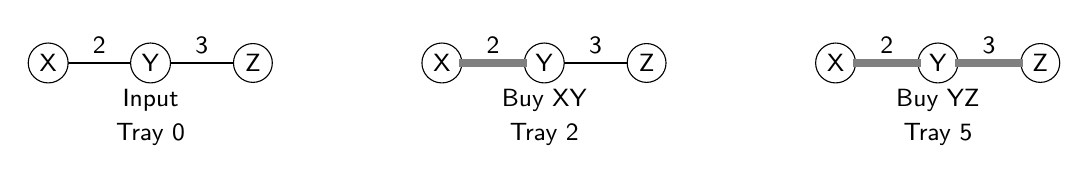
\begin{tikzpicture}[x=1cm,y=1cm, every node/.style={font=\small}]
\foreach \offset/\caption in {0/Input,5/Buy XY,10/Buy YZ}{
 \begin{scope}[xshift=\offset cm]
 \draw (0,0)--(1.3,0)--(2.6,0);
 \node[above] at (.65,0){2}; \node[above] at (1.95,0){3};
 \foreach \x/\s in {0/X,1.3/Y,2.6/Z}{\node[circle,draw,fill=white,inner sep=2pt] at (\x,0){\s};}
 \node at (1.3,-.48){\caption};
 \end{scope}}
 \draw[line width=3pt,gray] (5.22,0)--(6.08,0);
 \draw[line width=3pt,gray] (10.22,0)--(11.08,0) (11.52,0)--(12.38,0);
 \node at (1.3,-.9){Tray 0};\node at (6.3,-.9){Tray 2};\node at (11.3,-.9){Tray 5};
\end{tikzpicture}
\end{center}
Trace X--Y--Z again: a bought network owes nothing more. Show returning a link and its refund. Introduce the next new action \emph{at its table}, using the printed start/step/result example: opening links (K--1 p.~2; middle p.~2; upper p.~3), trips (middle p.~3; upper p.~6), or squares (K--1 p.~4; middle p.~6; upper p.~8). For trips, record one word, then pay: on this line XYZ costs 5; XYZY costs 8. For squares, a pawn may pass through the square but need not visit it. Do not introduce three new objectives in one speech.

\textbf{Staffing and one hour.} Anchor one adult at each table; read or scribe without choosing links. In the trio rotate chooser, payer/checker and recorder. Use 5 minutes movement, 5 handling/launch, 20 exploring, 5 break, 20 continuing and 5 sharing. Young first route: P1--3; later P4--6, with P7--8 readiness-dependent. Middle: P1--3, then P4 if ready; save P5--8. Upper: P1--4, then one of P5--6; later P7--10, with P11--12 for proof-ready children. Finishing every page is not the goal.
\newpage
\head{K--1 solutions and discretionary hints}
AB means the whole link; buying it first or last does not make a new network. Spare record maps are workspace, not a promise of that many answers. Let children choose; the adult can read, count and draw their chosen links.

\sub{Problem 1 page 1}
Minimum \textbf{4}, exactly three networks: \links{AB, AC, CD}, \links{AB, BC, CD}, \links{AC, BC, CD}. D needs a link costing at least 2; two more links cost at least 1 each. Equality uses CD and any two sides of the A--B--C triangle. All three work, so the list is complete. \hint{``Can the pawn reach D? Which road could it use?''} If only one answer appears, ask whether the same payment pile can buy a different pair in the triangle.

\sub{Problem 2 page 2}
With 1-dot links open, groups are \textbf{AB / C / D / EF}; up to 2 dots, \textbf{ABC / DEF}; up to 3 dots, \textbf{ABCDEF}; up to 4 dots, still one group. The pawn first reaches F from A at \textbf{3}. Include isolated places in rings. Opening means marking every eligible link; no payment total is requested. \hint{``Where can the pawn go without crossing an unmarked road?''} A group need not look round; its membership matters.

\sub{Problem 3 page 3}
Minimum \textbf{9}, in two ways: \links{AB, AC, CD, DE, EF} and \links{AB, BC, CD, DE, EF}. The cheapest connecting price list is $1,1,2,2,3$: AB and EF are forced by their cheapest exits, DE joins D to E cheaply, and either AC or BC connects C. CD is the cheapest link between ABC and DEF. No network can avoid all 3- and 4-dot links, since the 1- and 2-dot links leave those two groups separate. \hint{``Can you cross from the left ring to the right ring without a 3 or 4?''}

\sub{Problems 4 and 5 pages 4 and 5}
Each outer triangle has three links priced 4. Without S, any two cost \textbf{8}, the minimum. For P4, using S costs \textbf{6}, uniquely AS, BS, CS. For P5's top map, using S costs \textbf{9}, uniquely the three spokes: the square costs one extra. On P5's bottom map, using S costs \textbf{8}: AS, BS together with \emph{one of} CS, AC or BC. The square ties rather than saves. Those are all three cheapest ways using S; adding the three outer pairs gives six cheapest overall.

Why complete: a cheapest join using S is a tree. It uses three spokes, two spokes and one outer link, or one spoke and two outer links. Comparing these three forms gives the stated minima. The last form is wasteful when S is optional, but it must not be silently forbidden in a comparison that requires using S. \hint{P4: ``Do all three circles have to use an outside road?'' P5: ``Must using the square mean buying all its roads?''} Keep both piles for these small comparisons.

\sub{Problem 6 page 6}
Without X: \textbf{12}, any three outer sides (four choices). Using X: \textbf{8}, uniquely AX, BX, CX, DX, saving 4. Without X, a four-place tree needs three price-4 links. With X, a spanning tree on five places needs four links, each at least 2; four spokes attain that bound. \hint{``How many circles can your marked roads reach?''} If ready, ask whether any other four-link purchase can still cost 8.

\newpage
\head{Young continuation and middle entry}
\sub{K--1 Problem 7 page 7}
Minimum \textbf{6}, uniquely AS, BS, ST, CT, DT. Without either square the cost is 10 (AB, AC, CD); allowing only S or only T lowers it to 9. With both, five links are needed and only four price-1 links exist, so cost is at least $1+1+1+1+2=6$. \hint{``What would join the two small groups through their squares?''} This is a continuation, not a required young-table proof.

\sub{K--1 Problem 8 page 7}
Use positive whole-number dots. A working answer is \textbf{2, 2, 4} on the three spokes; 1, 3, 4 and 2, 3, 3 also work, in any arrangement. Complete rule: sort the spoke prices $x\le y\le z$. The cheapest join using S costs $\min(x+y+z,x+y+4,x+8)$. It equals 8 exactly for \textbf{$(1,3,z)$ or $(2,2,z)$ with $z\ge4$, or $(2,3,3)$}. Do not cap invented dots unless reducing the task deliberately. \hint{``Could two square roads and one outside road beat your three roads?''} A sum of 8 alone fails: 1, 1, 6 has a cost-6 alternative. The printed prompt leaves positivity implicit; say ``at least one dot per road'' before inventing prices.
\head{Grades 2--3 solutions and discretionary hints}
\sub{Problem 1 page 1}
Minimum \textbf{9}. Every cheapest network uses CD and EF, any two of AB, AC, BC, and one of CE, DE. The complete six are:
\begin{center}\small
\begin{tabular}{ll}
AB, AC, CD, CE, EF & AB, AC, CD, DE, EF\\
AB, BC, CD, CE, EF & AB, BC, CD, DE, EF\\
AC, BC, CD, CE, EF & AC, BC, CD, DE, EF
\end{tabular}
\end{center}
The three price-1 links chosen must join ABC and EF; CD is D's uniquely cheapest exit. A price-4 link is still needed between ABCD and EF, with two choices. The lower bound $1+1+1+2+4=9$ is attained in exactly those $3\times2$ ways. \hint{``Which part is still separate? Can two pairs share different triangle choices?''}

\sub{Problems 2 and 3 pages 1 and 2}
\begin{center}\small
\begin{tabular}{llll}
Pair & One lowest-dearest route & Dearest price & First common ring\\\midrule
A to D & ACD & 2 & 2\\
B to D & BCD & 2 & 2\\
D to F & DEF & 4 & 4\\
A to F & ACEF & 4 & 4
\end{tabular}
\end{center}
Other routes can be equally good; these problems do not request all routes. For P3: at price 1 the groups are \textbf{ABC / D / EF}; at 2, \textbf{ABCD / EF}; at 3, unchanged; at 4, one group. D is isolated below 2, and EF is separate below 4, proving the lower bounds. \hint{P2: ``Are we adding the prices or choosing the biggest?'' P3: ``Did the price-3 road actually join different groups?''}

\newpage
\head{Grades 2--3 trips and optional places}
\sub{Problem 4 page 3}
All three cheapest networks are AB, BC, CD. Their costs are \textbf{3, 6, 9} for original, +1 and +2 prices. Cheapest A--D trips are respectively \textbf{ABCD at 3; AD at 5; AD at 6}, each unique. These are the only two simple A--D routes; a repeated part costs extra. \hint{``Which roads stayed the same even though their total changed?''} Record links as well as costs, using the printed lines.

\sub{Problem 5 page 4}
All three cheapest networks are \textbf{AB, BC, CD, DE, EF}. Complete trip key:
\begin{center}\small
\begin{tabular}{llll}
Prices & Network cost & Every cheapest A--F trip & Trip cost\\\midrule
Original & 8 & ABCDEF, ACDEF & 8 each\\
Every price 2 more & 18 & ACDF & 15\\
Doubled & 16 & ABCDEF, ACDEF & 16 each
\end{tabular}
\end{center}
For the network, AB, BC, CD, DE, EF are uniquely cheapest across cuts A / rest, AB / rest, ABC / DEF, ABCD / EF and ABCDE / F respectively. For trips, both original ways to reach C cost 3; then CDE costs 3 and EF costs 2. After +2, AC wins to C and DF wins from D to F. Guide p.~7 gives a complete shortest-trip certificate. \hint{``Can a road we did not buy still be used on a trip?''} Yes: a trip is on the whole printed map. Reuse counters between the 18/15 and 16/16 comparisons.

\sub{Problems 6 and 7 page 5}
P6: write AB$=a$, BC$=b$, AC$=c$, using positive whole numbers. For a \emph{strict} switch, $a+b<c<a+b+2$, hence \textbf{$c=a+b+1$}. For example 1, 1, 3; 1, 2, 4; 2, 2, 5. The two-link trip gains 4 while the direct trip gains 2. \hint{``How much did each trip gain?''} If a child allows tied cheapest trips, $a+b\le c\le a+b+2$ also meets a weak reading of the prompt; ask whether they intended a tie or a clear switch, rather than rejecting it.

P7: \textbf{No; no}, for the no-square maps used so far and changes keeping prices positive. Every connecting tree has the same number of links, so adding the same amount preserves its ranking; doubling doubles every trip total. \hint{``Do all networks gain the same number of extra counters? Do all trips?''} P8 changes the rules, so the first answer need not survive there.

\sub{Problem 8 page 6}
Left: \textbf{8 without S, 6 using S}. Right: \textbf{8 without, 9 using}. Without, choose any two outer links; using, the unique minimum is AS, BS, CS on each map. The three tree forms on guide p.~3 prove the comparisons. \hint{``Is an optional place always a bargain?''} Let the child demonstrate the two piles before discussing a general rule.
\newpage
\head{Grades 4--5 routes groups and general claims}
\sub{Problem 1 page 1}
The answers are \textbf{A--D 2 via ACD; B--D 2 via BCD; D--F 4 via DEF; A--F 4 via ACEF}. Other routes are valid. D cannot be reached below 2; crossing between ABCD and EF requires at least 4. \hint{``Which groups would remain apart if that largest price were forbidden?''}

\sub{Problem 2 page 2}
Minimum \textbf{9}, exactly the six networks listed under middle P1 on guide p.~4. In each choose two of AB, AC, BC, then CD, EF and one of CE, DE. The product of three triangle choices and two bridge choices proves completeness; buying order is irrelevant. \hint{``Can you organize the records by what changes near A, then by what changes near E?''} Pool the six cases across the trio.

\sub{Problem 3 page 3}
At thresholds 1, 2, 3, 4 the groups are \textbf{ABC / D / EF; ABCD / EF; ABCD / EF; ABCDEF}. Starting with no open links gives six groups, so counts $c_0,\ldots,c_4$ are \textbf{6, 3, 2, 2, 1}. The first common thresholds for A--D, B--D, D--F, A--F are \textbf{2, 2, 4, 4}. Opening the price-3 link changes no group. \hint{``If a road opens inside one ring, does the number of groups change?''} Isolated places still count as groups.

\sub{Problem 4 page 4}
Minimum \textbf{6}, exactly three networks:
\begin{center}
\links{AB, AC, CD, DE}\qquad\links{AB, BC, CD, DE}\qquad\links{AC, BC, CD, DE}.
\end{center}
At price 1 the groups are \textbf{ABC / D / E}; at price 2 all five places join, and later thresholds do not change that. All three networks have prices \textbf{1, 1, 2, 2}. A five-place tree needs four links. Only two price-1 triangle links can be used without a loop, so cost is at least $1+1+2+2=6$. CD and DE are the only price-2 links; the three triangle pairs complete the list. \hint{``Can three price-1 links help reach D or E?''}

\sub{Problem 5 page 5}
\textbf{Sam is wrong.} Every loop-free connecting network on the square uses three sides and has largest price 3. The network BC, CD, AD costs \textbf{9}; each of the other three costs \textbf{7}, using AB and any two of BC, CD, AD. Largest price 3 is unavoidable but does not determine total cost. \hint{``Can two networks have the same dearest road and different payment piles?''} Distinguish Sam's one number for the whole network from P6's condition for every pair.

\sub{Problem 6 page 5}
\textbf{Yes; no; yes}, on a connected positive-price map with no squares. Every cheapest-network route is lowest-dearest; all cheapest networks have the same price list; threshold groups determine cost. The proof ideas open this guide. Two examples suggest, but do not prove, a universal statement.

For P2--3 the group drops are $6-3=3$, $3-2=1$, $2-2=0$, $2-1=1$. Therefore there are \textbf{three price-1 links, one price-2 and one price-4}, giving $3+2+4=9$. Alternatively add $5+2+1+1=9$. For P4, the drops are $5-3=2$, $3-1=2$, giving $2+4=6$, or $(5-1)+(3-1)=6$. Count the threshold-3 pause in the first map even though no link of that price is bought.

\hint{``Suppose a cheaper-dearest route existed. What happens if we lift the dearest road in your tree?''} Draw the two resulting sides and let the child find where the proposed route crosses. For the price-list question ask, ``How many links are needed inside each ring?'' Save the converse for P12.

\textbf{Limit.} P9's 2,2,4-spoke map has cheapest lists 4,4 and 2,2,4: optional squares change the theorem.
\newpage
\head{Grades 4--5 trips and optional places}
\sub{Problem 7 page 6}
Networks are \textbf{AB, BC, CD} in all three maps, costing \textbf{3, 6, 9}. Cheapest trips are \textbf{ABCD at 3; AD at 5; AD at 6}. Each is unique: the two simple routes compare $3$ with $4$, $6$ with $5$, and $9$ with $6$. \hint{``Which payment counts every bought road, and which counts only your trip?''} Reuse the printed trip example before comparing totals.

\sub{Problem 8 page 7}
Every cheapest network is \textbf{AB, BC, CD, DE, EF}, uniquely. The cut argument under middle P5 proves this, and strictly increasing changes preserve all its strict comparisons.
\begin{center}\small
\begin{tabular}{llll}
Prices & Network cost & Every cheapest A--F trip & Trip cost\\\midrule
Original & 8 & ABCDEF, ACDEF & 8 each\\
Every price 2 more & 18 & ACDF & 15\\
Every price doubled & 16 & ABCDEF, ACDEF & 16 each\\
Each price times itself & 14 & ABCDEF & 14
\end{tabular}
\end{center}
\textbf{Complete trip certificate.} The least costs from A to A,B,C,D,E,F are respectively
\[
\begin{array}{c|rrrrrr}
 &A&B&C&D&E&F\\\hline
\text{original}&0&1&3&5&6&8\\
+2&0&3&5&9&12&15\\
\times2&0&2&6&10&12&16\\
\text{squared}&0&1&5&9&10&14
\end{array}
\]
Every printed link satisfies $d(v)\le d(u)+w(uv)$ in both directions; summing along a route proves its cost is at least the destination label. The listed trips attain the bound. Equality requires each step to advance by exactly its price: originally C can follow either A or B, while D, E, F must follow C, D, E; after +2 the successful chain is A,C,D,F; doubling keeps the original choices; squaring forces A,B,C,D,E,F. Thus no cheapest trip is missing. These adult labels are not an extra child ledger.

None of the three changes alters cheapest \emph{all-place} networks. Addition and squaring can change cheapest trips; doubling cannot. \hint{``What does adding 2 do to a three-road trip compared with a five-road trip?''} For squaring ask which costly single road now competes with several cheaper ones. Never ask the kit to pay the squared price 36; numerical comparison is enough.

\sub{Problem 9 page 8}
\textbf{Left star: cost 8, three ways}, AB/AC, AB/BC, AC/BC; S is unused. A tree using S costs at least 9. \textbf{Right star: cost 8, six ways}: those same three outer pairs, plus \links{AS, BS, CS}, \links{AS, BS, AC}, \links{AS, BS, BC}. The three tree forms from guide p.~3 show completeness. \textbf{Bottom map: cost 8, two ways}, \links{AB, BC, CD, DE, EF} and \links{AC, CD, DE, EF}. Only A and F are circles; B,C,D,E are squares. A positive-price optimum for two required endpoints is just a cheapest simple trip, so P8's original trip list proves completeness. \hint{``Which places must be reached here? Could you return a road that goes only to an optional dead end?''}

\sub{Problem 10 page 9}
Cheapest is \textbf{6}, uniquely AS, BS, CS. From AB and BC, the answer is \textbf{no}: with a cap of 8, a purchase with no spoke can only be an outer pair. Returning a link disconnects a circle; buying any link exceeds 8; swapping an outer link for one spoke still disconnects a circle. Only swaps to the other outer pairs survive. The same holds with cap 9. A cap of \textbf{10} is enough: buy AS (10), swap AB for BS (8), swap BC for CS (6). \hint{``Could one new spoke connect both sides left by returning an outside road?''} A swap is one atomic exchange; its final state must connect the circles. This optional-place example, not a contradiction, marks the limit of the first-visit exchange test.
\newpage
\head{Upper continuations explanations and sources}
\sub{Problem 11 page 10}
Minimum \textbf{6}, uniquely AS, BS, ST, CT, DT, as in young P7 (guide p.~4). A square place cannot have just one bought link in an unrestricted cheapest purchase: that link is a positive-price dead end, removable without separating any required circle. A square can be unused (degree zero); do not confuse that with an optional leaf in the bought tree.

With four circles, the largest possible number of squares with three or more bought links is \textbf{2}. This map attains it at S and T. Here is a proof that also covers larger maps. Ignore unused places. A cheapest purchase is a tree; every leaf is required. If there are $L$ leaves and the branch places have degrees $d_1,\ldots,d_b\ge3$, counting link ends gives
\[
 -L+\sum_{i=1}^{b}(d_i-2)=-2,\qquad
 L=2+\sum_{i=1}^{b}(d_i-2).
\]
Degree-2 places add nothing. Each branch place accounts for at least one extra leaf beyond two, so there are at most $L-2$ branch places altogether. Since $L\le4$, at most two can be optional branch places. More generally $r$ required places give at most $r-2$ such squares, for $r\ge2$.

\hint{``What happens to the payment if we return the only road to that square?''} For the bound, ask, ``When a path splits again, how many extra ends must eventually appear?'' Children may explain with drawn branches; algebra is adult backup. Two branches on this particular map show attainability, not by themselves a universal bound.

\sub{Problem 12 page 10}
\textbf{Lee is right}, for a connected map with no squares and positive prices. His condition implies every unused link $f$ costs at least every link on the candidate tree route between its ends: $f$ itself is an available route. This is the exchange certificate. The following transformation proves its sufficiency without assuming a buying algorithm.

Let T be Lee's tree and R any competing spanning tree. Choose a link $e$ of T missing from R. Deleting $e$ splits T into two sides. Adding $e$ to R makes a loop; some other loop link $f$ crosses those sides. The only T link across that split was $e$, so $f$ is not in T. The T route between $f$'s ends uses $e$, and Lee's condition gives $w(e)\le w(f)$. Replace $f$ with $e$ in R: cost cannot rise, and agreement with T increases. Repeat until R becomes T. Thus T costs no more than any spanning tree; any connected purchase with loops can first shed positive-price links. T is globally cheapest.

\hint{``What does Lee's condition say about a route consisting of just one unused road?''} If the full transformation is too abstract, enact one exchange, retain the conjecture, and save the proof. Sam's claim in P5 checks only the whole network's largest price; Lee checks every pair, a much stronger condition.

\sub{Sources consulted and boundaries}
{\small
Consulted: the final three student PDFs (W53-RV-K/M/U-v1), editable sources, earlier page reviews, return-visit README and \texttt{week-53-return-visit.md} outline; base Week 53 guide, especially pp.~1--2 and its exchange argument; Week 8 return-visit and Week 98 model guides. Old review numbering predates the revised pages; this guide and its independent checker use the final PDFs.

The outline cites T. C. Hu, ``The Maximum Capacity Route Problem,'' \textit{Operations Research} 9(6), 1961, pp.~898--900 (only its abstract checked by the outline author); Sedgewick and Wayne, \textit{Algorithms}, 4th ed., \S4.3 companion, Exercise 1 and Web Exercise 1 (repricing and bottleneck distinction); and the Wikipedia articles ``Widest path problem'' and ``Steiner tree problem.'' Hwang, Richards and Winter, \textit{The Steiner Tree Problem}, 1992, is background cited there, not consulted here. Those originals were not reconsulted; this guide supplies elementary proofs and independent finite checks.

Base-week research notes give the activity lineage: CS Unplugged Activity 9, ``The Muddy City,'' printed pp.~76--80, PDF pp.~1--5, and \textit{Math Circle by the Bay}, ``How we teach,'' printed p.~ix/PDF p.~10. The notes, not those unavailable originals, were consulted. Materials and pacing are untested proposals. Record pages used, handling problems and adult decisions needed.
}
\end{document}
